\setchapterpreamble[u]{\margintoc}
\glsresetall % reset glossary

\chapter{Literature review}
This thesis focuses on numerical optimization in the structural engineering domain. As such, one needs familiarity with existing optimization methods and contemporary engineering practices. The purpose of this chapter is to provide the reader with a non-exhaustive historical overview of structural optimization, particularly in the context of ultralight and modular structures. Additionally, we introduce crucial concepts and terminology that will be employed consistently throughout the document.

\section{An introduction to structural optimization}
Structural optimization is a multidisciplinary field within engineering that aims to systematically improve structural performance--considering factors like mass, stiffness, and dynamic response--by optimizing their shape, material distribution, and overall design. Historically, structural optimization algorithms are categorized into three families: sizing, shape, and topology optimization. Sizing optimization concentrates on determining the optimal distribution of variables, where both the design and state variable domains are known \textit{a priori} and remain constant during optimization. In contrast, shape optimization aims to discover the optimal shape of a predefined domain, treating the domain itself as a design variable allowing for flexibility in shaping the structure. Topology optimization goes further, involving the determination of features like the number, location, and shape of holes, as well as the connectivity of the structural domain. This approach offers a more comprehensive exploration of possibilities in structural design. A visual representation of the three families is provided in \figref{fig:02_opt_fam}.

\begin{figure}
    \centering
    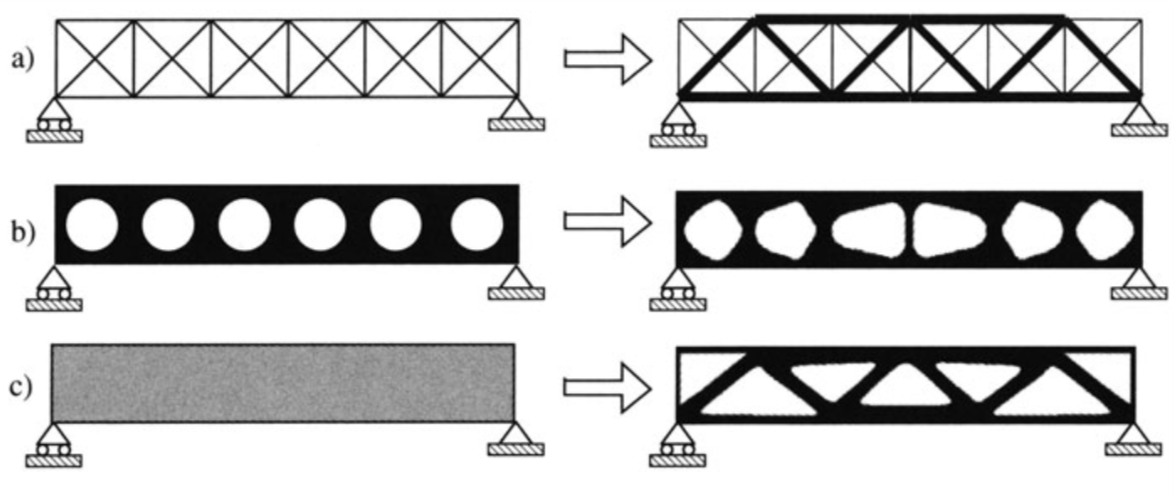
\includegraphics[width=\linewidth]{figures/02_literature/opt_family.png}
    \caption{Visual representation of (a) size, (b) shape, and (c) topology optimization \cite{bendsoe_topology_2004}.}
    \label{fig:02_opt_fam}
\end{figure}

Structural optimization involves using mathematical algorithms, computational models, and iterative analyses to explore and refine design solutions. For that reason, we introduce the basic concepts and terminology behind numerical optimization. In numerical optimization, algorithms are employed to minimize or maximize a specific function by adjusting various design variables. The problem may or may not be subject to constraints. Formulating an optimization problem is a crucial step to prevent common conceptual errors, such as confusing constraints with objective functions. An incorrect problem formulation can lead to a failed solution or yield a mathematical optimum that lacks feasibility from an engineering perspective.

The most general formulation of an optimization problem is written as:
\begin{equation}
    \begin{aligned}
    \min_{\vect{x}}         && & f(\vect{x})\\
    \textrm{by varying}   && \vect{x} &\in [l^-,l^+] \\
    \textrm{s.t.}   && \vect{g}_\text{e}(\vect{x}) &= 0 \\
    && \vect{g}_\text{i}(\vect{x}) &> 0, \\
    \end{aligned}
\end{equation}
where $ f(\vect{x}) $ is the objective function to minimize, $ \bm{x} $ is the vector of design variables bounded between $ l^- $ and $ l^+ $, and $\vect{g}_\text{e}$ and $\vect{g}_\text{i}$ represent the equality and inequality constraints, respectively.

\paragraph{Objective Function}
In numerical optimization, the objective function $f(\vect{x})$ represents the scalar that we aim to minimize. Should the goal be to maximize a function, one can achieve this by minimizing the opposite of that function, maintaining adherence to the convention. Common objective functions in structural design include the minimization of volume or structural compliance. The objective function can take the form of an explicit function or result from a highly complex computational procedure. The selection of the objective function is crucial to propose a design that is feasible from an engineering perspective, regardless of the precision of the optimization scheme employed.

Optimization problems are categorized in the literature based on how the objective function is with respect to design variables, whether linear, quadratic, or generally non-linear. It is possible to concurrently optimize multiple objective functions, but this usually results in a family of optimum designs with differing emphases on the various objectives called the Pareto front. When possible, it is more straightforward to convert these diverse objectives into constraints~\sidecite{martins_engineering_2021}.

\paragraph{Design Variables}
The design variables $\vect{x}$ are the parameters that the optimizer algorithm changes to minimize the objective function. Design variables could be continuous or discrete if only some distinct values are allowed (for example, only a certain size for a hole in a structural analysis). The optimization problem formulation allows for the lower and upper boundary for each design variable known in the literature as variable bounds.

\paragraph{Constraints}
The constraints are functions used to restrict the design variables in some way. They serve the purpose of preventing the algorithm from converging to a numerical minimum that is not feasible due to physical and engineering constraints. Similar to the objective function, constraint functions can take on linear, quadratic, or generally non-linear forms, and different algorithms must be applied accordingly.

Constraint functions can be further classified into two types: equality constraints ($\vect{g}\text{e}$), which arise when the design variables are restricted to be equal to a fixed quantity, and inequality constraints ($\vect{g}\text{i}$), which come into play when the design variables are required to be greater than or equal to a certain quantity.

\subsection{Optimizers}
The field of numerical optimizers is extensive. For that reason, our focus here will be specifically on algorithms employed in structural optimization. Various algorithm types have been applied to address structural optimization problems, predominantly categorized into three main families: optimality criteria, metaheuristic algorithms, and gradient-based strategies.

\gls{oc} refer to mathematical conditions or rules used to assess and guide the modification of a design or structure to achieve the desired performance~\sidecite{prager_problems_1968,prager_optimality_1968}. In the context of topology optimization, \gls{oc} are primarily applied in compliance minimization problems, as each element contributes independently to the overall compliance. Bendsøe used \gls{oc} to seek the stiffest plate \ie compliance minimization--that can be made of a given amount of material and, together with Kikuchi~\sidecite{bendsoe_generating_1988}, they used \gls{oc} to obtain optimal shape design of structural elements based on boundary variations without the use of remeshing. Later, Bendsøe and Sigmund~\sidecite{bendsoe_optimization_1995,sigmund_99_2001} introduced a heuristic update scheme for isotropic materials, while Allaire \etal~\sidecite{allaire_homogenization_1996} demonstrated the convergence proof for both isotropic and anisotropic materials using the \gls{ad} approach. In both methods mechanical analysis provides essential information for solving closed-form conditions, allowing iterative updates of variables until convergence is achieved. Recently, \gls{oc} methods gained interest again thanks to the reduced calculation time~\sidecite{li_accelerated_2020, ferrari_new_2020} thanks to a modified Anderson acceleration strategy~\sidecite{anderson_iterative_1965}.

Metaheuristic (or gradient-free) algorithms offer a broader range of options compared to their gradient-based counterparts. While gradient-based algorithms typically conduct local searches, possess mathematical justification, and operate deterministically, metaheuristic algorithms are simpler and usually take much less developer time to use, and are perfect candidates for smaller problems. They find very diverse application cases and are useful when the design space is discrete, with multiple objective functions, or highly non-linear with many local minima (multimodal). The works authored by Conn \etal~\sidecite{conn_introduction_2009} and Audet and Hare~\sidecite{audet_derivative-free_2017} offer a comprehensive exploration of gradient-free optimization algorithms. Evolutionary algorithms, a prominent category, simulate natural selection by retaining the fittest solutions in each generation while introducing mutations or cross-overs for improvement. A review of these optimization methods is given in the following reference~\sidecite{simon_evolutionary_2013}. These algorithms, also called \gls{ga}, are employed for example by Balamurugan \etal~\sidecite{balamurugan_two_2011} for compliance minimization, showcase versatility but face challenges with combinatorial considerations as the number of design variables increases~\sidecite{sigmund_usefulness_2011}. Particle swarm and ant colony algorithms, inspired by nature, provide alternative strategies with randomness and new search directions. However, these non-gradient methods require regularization schemes for topology optimization, as outlined by Luh, Lin, and others~\sidecite{luh_structural_2009, luh_binary_2011}.
Targeting the resolution of \gls{mip} problems, branch-and-bound algorithms divide the feasible set of the original problem into subsets through a process known as branching. These subsets are then further segmented to refine the partition of the feasible set. For each subset, lower bounds and optionally upper bounds on the objective function value are determined, a process referred to as bounding. Typically, the lower bounding problems are convex problems that can be efficiently solved to global optimality. Stolpe~\sidecite{stolpe_global_2004} addresses a volume minimization problem on a truss using a continuous branch-and-bound method, ensuring convergence to a globally optimal solution. The \gls{eso} framework, initially a metaheuristic, removes less solicited elements iteratively~\sidecite{mattheck_new_1990, xie_simple_1993}. These methods offer freedom in optimization and improved convergence to local minima, especially in handling various optimization problems like buckling~\sidecite{manickarajah_evolutionary_1998}. The \gls{eso} algorithm has been enhanced by the \gls{beso} framework~\sidecite{young_3d_1999}, which allows both removal and addition of elements. 

Gradient-based algorithms in optimization leverage local information at a trial point to comprehend the shape of the local objective function in the neighborhood. This insight is crucial for determining the optimal direction to minimize the objective function. Typically, only the Jacobian (first derivative) is utilized, though more advanced algorithms incorporate the Hessian (second derivative). The computational demand for gradient calculation often constitutes the most resource-intensive aspect of the optimization loop. When constraints are present, solving the problem directly on the analytic response surface of the objective function becomes impractical. Consequently, the approach involves creating local approximations of the problem at the current design point using gradient information. These approximations are designed so that specialized algorithms can efficiently solve them. The categorization of gradient-based algorithms is often based on how this local approximation is constructed.

The most used approximations in structural optimization includes among others \gls{slp}, \gls{sqp} and \gls{slsqp}~\sidecite{kraft_software_1988}, \gls{mma}~\sidecite{svanberg_method_1987} and its amelioration \gls{gcmma}~\sidecite{svanberg_class_2002} and \gls{gbmma}~\sidecite{bruyneel_family_2002}, and \gls{conlin}~\sidecite{fleury_structural_1986}. Specialized algorithms for solving the approximated problems are, among others, the primal-dual method and interior-point method.

An interior-point method is a numerical optimization algorithm used to solve constrained optimization problems. The key idea behind interior-point methods is to transform the constrained optimization problem into a sequence of unconstrained problems, allowing for efficient iterative solutions. The method introduces a barrier function that penalizes points outside the feasible region, effectively creating a "barrier" against leaving that region. This barrier function is incorporated into the objective function, and as the optimization progresses, it guides the search towards the interior of the feasible region. The term "interior point" originated from early methods that relied on interior penalty techniques, assuming the initial point was feasible. Nevertheless, contemporary interior-point methods such as the open source IPOPT~\sidecite{wachter_implementation_2006} are more versatile and can start from infeasible points. Rojas Labanda and Stolpe conducted a benchmark of various optimization algorithms and structural optimization formulations using a compliance minimization problem. Their findings highlight the efficacy of employing interior-point algorithms such as IPOPT in topology optimization problems~\sidecite{rojas_labanda_benchmarking_2015}.

\section{Ultra-lightweight structures optimization approaches}
Two of the most frequently employed formulations for structural optimization are the minimization of volume while adhering to stress constraints and the minimization of compliance under volume constraints. Historically, the volume minimization formulation has been used in the first works of structural optimization of truss structures~\sidecite{dorn_automatic_1964,chan_optimum_1964,hemp_optimum_1973}. The problem was initially formulated in terms of member forces, ignoring the kinematic compatibility to obtain a \gls{lp} problem. The formulation was modeled using the \gls{sand} approach, in which the equations of nodal equilibrium are treated as equality constraints, and where both nodal displacements and the cross-sectional areas of truss members serve as design variables~\sidecite{sankaranarayanan_truss_1994}. These methods are known in the literature as layout optimization or \gls{tto}. 

However, to attain greater design freedom, the structure optimization field later transitioned from truss structures to continuous discretization (also called density methods). While truss structures offered simplicity and ease of analysis, they imposed limitations on the design due to their discrete member configurations and their inability to transmit moments, handle torsional effects, and represent complex structural elements such as plates or volumes. The continuum mesh offered instead more versatility~\sidecite{bendsoe_generating_1988,bendsoe_optimal_1989}, and has since been used for multiple different applications, \eg the design of optimized repetitive metamaterials~\sidecite{sigmund_materials_1994, zhang_scale-related_2006,collet_topology_2018}, fluids optimization~\sidecite{borrvall_topology_2003}, modelization of self-weight of the structure~\sidecite{bruyneel_note_2005}, the simulation of advanced manufacturing constaints~\sidecite{sigmund_manufacturing_2009,brackett_topology_2011}, the design of compliant mechanism~\sidecite{sigmund_design_1997, bruns_topology_2001}, or the optimization for additive manufacturing~\sidecite{wang_space-time_2020}. Other than the density methods, other ways to deal with topology optimization exist, like level-set methods \sidecite{allaire_level-set_2002,wang_level_2003,allaire_structural_2004}. The \gls{sand} approach is, however, incompatible with continuum meshes due to its excessive number of variables\sidenote{This proposition holds when referring to the end of the 1980s when computational power was scarce compared to what we have today.}. Given this limitation, a new approach was required to better handle the complexity of continuum meshes.

In the density-based \acrfull{nand} approach, the nodal displacement (state) variables are eliminated from the optimization problem through a process where the structural equilibrium equation is solved every iteration instead of being used as a constraint of the optimization. This results in an independent nested phase where the state equation of structural equilibrium is solved separately from the optimization algorithm. This creates a dense coupling between displacement and material density variables, necessitating a computationally expensive sensitivity analysis within the nested algorithm, typically employing the adjoint method (more information about the adjoint method on the following resurces~\sidecite{tortorelli_design_1994,martins_engineering_2021}). Nevertheless, if the problem is reformulated as a compliance minimization with volume constraints, the problem is self-adjoint and the adjoint algorithm is no longer necessary to evaluate the gradient sensitivities~\sidecite{bendsoe_topology_2004}, and this reduces considerably the computational times.

Both the \gls{tto} methods based on the ground structure and the density-based topology optimization approaches are good candidates for the optimization of ultra-light structures. We review here their main characteristics and numerical properties, starting from density-based approaches.

% The introduction of new propulsion technologies (electric, LH2) aimed at reducing greenhouse gas emissions in the aeronautical sector provides an opportunity to rethink the structure design from the initial phases. The subsequent reevaluation of associated design methods has led to the exploration of structural optimization techniques. Topology optimization, in particular, offers a valuable approach to identifying optimal shapes and material distributions and allows achieving any shape within the design space instead of dealing with predefined configurations. Classical topology optimization considers the design domain as a continuum, in which each location may or may not have a material assigned to it~\cite{bendsoe_optimal_1989}. While topology optimization offers tremendous benefits in terms of weight reduction and structural efficiency, it is important to acknowledge the challenges associated with manufacturing such designs. The intricate and complex geometries generated through the optimization can pose difficulties in the fabrication process, often requiring advanced manufacturing techniques, specialized equipment, and specific constraints in the optimization \cite{zhou_progress_2002,brackett_topology_2011,liu_current_2018}. Additionally, the computational time required for generating such optimized designs, particularly for low-volume fractions typical of the aerospace domain, can be significant \cite{aage_giga-voxel_2017}, impacting the overall efficiency of the design process. This remains true even with the use of adaptive meshes~\cite{salazar_de_troya_adaptive_2018, zhang_adaptive_2020}.

\subsection{Density-based topology optimization}

\begin{marginfigure}
    \centering
    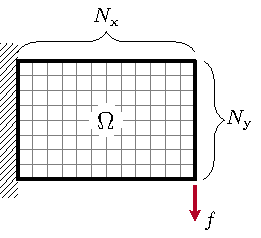
\includegraphics{figures/02_literature/01_contin_mesh/c_mesh.pdf}
    \caption{The domain $\Omega$ is discretized using $N_\text{e}=N_\text{x} N_\text{y}$ continuous 4-nodes elements.}
    \label{fig:02_mesh_c}
\end{marginfigure}
Let $\Omega \in \mathbb{R}^2$ be a rectangular domain of dimensions $X$ and $Y$, containing respectively $N_\text{x}$ and $N_\text{y}$ linear 4-nodes elements, for a total of $N_\text{e}=N_\text{x} N_\text{y}$ elements and $M$ nodes (see \figref{fig:02_mesh_c}). The objective of the optimization is the minimization of the compliance $C$ of the structure, equivalent to finding the structure with the least possible nodal displacement with respect to a defined set of boundary conditions. 

\paragraph{Compliance minimization formulation} The Problem $\mathbb{T}_0$ is stated in terms of the design variables $\vect{\rho}$ as follows:
\begin{equation}
    \begin{aligned}
    \min_{\vect{\rho}}         && C &= \sum_{i} \vect{u}_{e,i}^T \matr{K}_{e,i} \vect{u}_{e,i}=\vect{f}^T\vect{u}&& \forall i \in [0,\dots,N_\text{e}]                         \\
    \textrm{s.t.}   && & \frac{1}{V_\text{p}}\frac{\sum_{i} \left(\rhophys_i v_i \right)}{V_0} - 1 \leq 0 && \forall i \in [0,\dots,N_\text{e}] \\
    && \matr{K}\vect{u} &= \vect{f} &&\\
    && 0 &\leq \rho_i \leq 1. && \forall i \in [0,\dots,N_\text{e}] \\
    \end{aligned}
    \tag{$\mathbb{T}_0$}
    \label{eq:02_prob-comp}
\end{equation}
The design variables $\vect{\rho}$ are defined for every element of the structure as $\vect{\rho} = [\rho_1, \rho_2, \ldots,\rho_{Ne}]^T$, with $\rho_i \in [0,1], \; \forall i \in [0,\dots,N_\text{e}]$. The physical densities $\vect{\rhophys}$ are related to the design variable $\vect{\rho}$ through density filtering and threshold projection~\sidecite{wang_projection_2011}, as explained later in the document. $V_\text{p}$ is the prescribed volume fraction that acts as the constraint of the minimization problem, while $v_i$ represents the area of the $i$-th element and $V_0$ is the total area of the domain $\Omega$. $\matr{K}\vect{u} = \vect{f}$ is the state equation of the problem and defines the elastic response of the structure to an external nodal load $\vect{f}=[f_1, f_2, \ldots,f_{2M}]^T$. The global stiffness matrix $\matr{K}$ is assembled from the element stiffness matrix $\matr{K}_{e,i}$ and $\matr{K}_{e,i} = E_i \matr{K}_{e,0}$ where $\matr{K}_{e,0}$ represents the element stiffness matrix relative to the chosen type of element (linear or quadratic) and $E_i(\rhophys_i)$ the Young's modulus of the $i$-th element. 

The material scheme used to interpolate between void and full material is the well-known \gls{simp}~\sideciteonce{bendsoe_optimal_1989,bendsoe_material_1999} approach. It is governed by the equation:
\begin{equation}
    E_i(\rhophys_i) = E_{\textrm{min}} + \rhophys_i^p(E_0-E_{\textrm{min}}),
    \label{eq:02_simp}
\end{equation}
where the parameter $p$ penalizes the intermediate densities and pushes the result to a black-and-white result. $E_0$ is the Young's modulus of the dense material and $E_{\textrm{min}}$ is a small value used to avoid the global stiffness matrix $\matr{K}$ from being singular when $\rhophys_i=0$. 

The \gls{simp} exponent $p$ is constrained to be greater than or equal to 1. From a physical perspective, the extreme case of $p = 1$ makes sense only in a two-dimensional optimization context, where it becomes equivalent to optimizing membrane thickness. When $p > 1$, the interpolation results in an equivalent homogenized stiffness tensor for intermediate densities, determined by the material-to-void ratio $\rho$. This mirrors microstructures conforming to the \gls{hs} conditions, which estimate the theoretical lower and upper bounds for the elastic modulus of a homogeneous, isotropic mixture of different materials based on their elastic modulus and volume fractions \sidecite{hashin_variational_1963}. If the exponent $p$ exceeds 3, Bendsøe \sidecite{bendsoe_material_1999} mathematically proves that the equivalent homogenized stiffness tensor adheres to the upper bound of the \gls{hs} conditions (refer to \figref{eq:02_simp}). It is important to note that in the mono-scale topology optimization context, deviating from the \gls{hs} bounds for intermediate densities is allowed. The objective is to drive the density distribution towards a black-and-white result with minimal intermediate densities, without concerning whether the equivalent homogenized stiffness tensor can be replicated by a real microstructure.

\begin{figure}
    \centering
    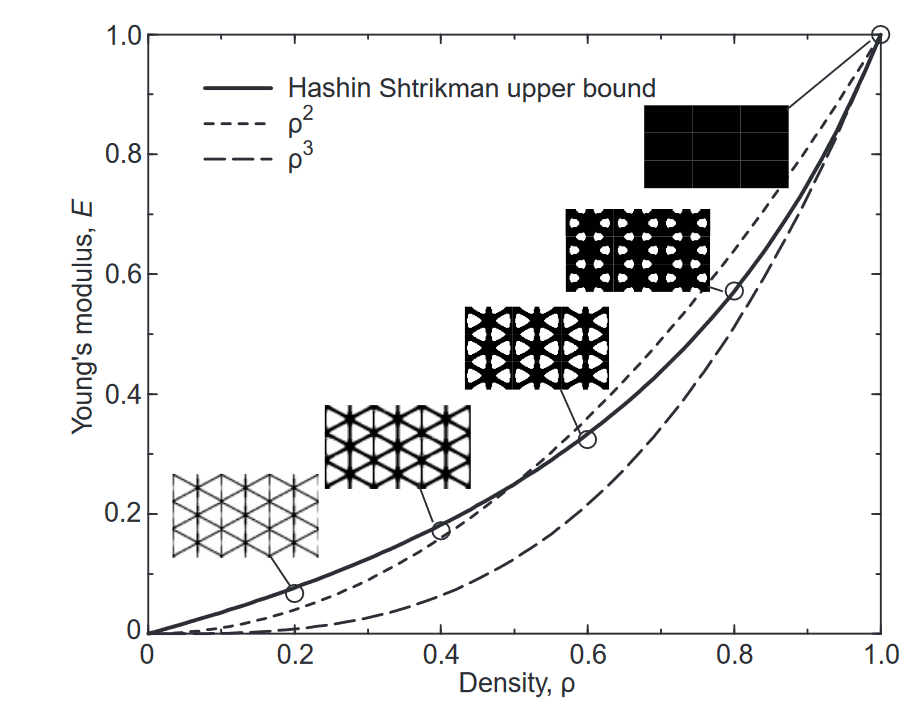
\includegraphics[width=0.75\linewidth]{figures/02_literature/simp.png}
    \caption{Comparison between SIMP model with the Hashin-Strikman upper bound, considering an isotropic material with a Poisson ratio of $1/3$ mixed with void. The Hashin-Strikman upper bound is illustrated with microstructures approaching the specified bounds. \cite{bendsoe_material_1999}.}
    \label{fig:02_simp}
\end{figure}

\paragraph{Spatial filtering and projection} 
Multiple approaches have been developed to solve the problems linked to mesh discretization, such as mesh dependency or the checkerboard problem~\sidecite{diaz_checkerboard_1995}. Filtering the sensitivity information of the optimization problem proved to be an effective approach to guarantee independence from mesh resolution~\sidecite{sigmund_design_1994,
sigmund_design_1997}. Another possibility is instead to directly filter the density field $\vect{\rho}$ using the 2D convolution operator~\sidecite{sigmund_morphology-based_2007}. The weight function $w$ (or kernel) of the convolution is defined as:
\begin{equation}
    w(d_j) = R - d_j, \quad j \in \mathbb{N}_{i,R}
\end{equation} 
where $\mathbb{N}_{i,R}$ represent the set of elements lying within a circle of radius $R$ centered on the $i$-th element and $d_j$ is the distance of the $j$-th element to the center of the filter (see \figref{fig:02_ker}).
\begin{marginfigure}
    \centering
    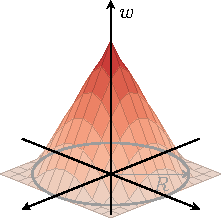
\includegraphics{figures/02_literature/02_circ_filter/filt_cir.pdf}
    \caption{Kernel of the 2D convolution operator.}
    \label{fig:02_ker}
\end{marginfigure} 
The filtered values $\vect{\rhofil}$ of the design variable $\vect{\rho}$  are calculated as:
\begin{equation}
    \rhofil_i = \frac{\sum_{j \in \mathbb{N}_{i,R}} w(d_j)v_j\rho_j}{\sum_{j \in \mathbb{N}_{i,R}} w(d_j)v_j}.
    \label{eq:02_rhofil}
\end{equation}
As the filtering phase produces a large number of gray elements, a smooth projection technique based on the \textit{tanh} function is implemented~\sidecite{wang_projection_2011} to evaluate the value of the physical density $\vect{\rhophys}$  of the structure:
\begin{equation}
    \rhophys_j = \frac{\tanh(\beta\eta)+\tanh(\beta(\rhofil_j - \eta))}{\tanh(\beta\eta)+\tanh(\beta(1 - \eta))},
    \label{eq:02_proj}
\end{equation}
where $\beta$ is a parameter that defines the slope of this approximation function: the larger the value of $\beta$, the fewer elements with intermediate density are present in the structure topology. $\eta$ is the threshold value of the projection.

In the domain of structural topology optimization, it is a widely adopted strategy to employ continuation methods. Introduced in the 90s \sidecite{allaire_numerical_1993, allaire_topology_1993}, they are used to converge towards more optimized structures. These methods solve a sequence of problems with increasing values of the \gls{simp} material penalization parameter $p$. Many researchers such as Bendsøe and Sigmund \sidecite{bendsoe_topology_2004} and Rozvany \sidecite{rozvany_critical_2009} consider, among others, continuation methods as a standard procedure in topology optimization. However, this approach comes at the expense of an increased number of iterations and, consequently, augmented computational time \sidecite{petersson_slope_1998}. In an effort to mitigate this drawback, Rojas Labanda and Stolpe \sidecite{rojas-labanda_automatic_2015} have derived an automatic penalization scheme. This innovative scheme aims to reduce both the objective function value and the number of iterations, providing an improvement over the classical formulation with a fixed penalty parameter. While the literature is predominantly focused on the continuation scheme on the \gls{simp} material penalization parameter $p$, it is worth noting that similar techniques could be employed for other optimization parameters \eg the filter radius $R$ or the projection parameter $\beta$.

While density-based topology optimization offers tremendous benefits in terms of weight reduction and structural efficiency, it is important to acknowledge the challenges associated with manufacturing such designs. The intricate and complex geometries generated through the optimization can pose difficulties in the fabrication process, often requiring advanced manufacturing techniques, specialized equipment, and specific constraints in the optimization~\sidecite{zhou_progress_2002,brackett_topology_2011,liu_current_2018}. Additionally, the computational time required for generating such optimized designs, particularly for low-volume fractions typical of the aerospace domain, can be significant~\sidecite{aage_giga-voxel_2017}, impacting the overall efficiency of the design process. This remains true even with the use of adaptive meshes~\sidecite{salazar_de_troya_adaptive_2018, zhang_adaptive_2020}. Even if the freedom of the design space offered by continuum meshes is high, it is known that at very low volume fractions (\eg ultralight structures), and, especially if buckling constraints and manufacturing considerations (\eg minimum length scale), are taken into account, the optimal topology resembles a truss-like structure~\sidecite{sigmund_non-optimality_2016}. As a result, a distinct branch of continuous topology optimization has emerged specifically tailored for optimizing truss-like structures, known as feature-mapping topology optimization (also called topology optimization with explicitly defined components).

\subsection{Feature-Mapping topology optimization}
Topology optimization methods using explicitly defined components have been developed to permit an easier interpretation of the solution, finding the optimal shape, size, and connectivity of components projected over a finite element continuum mesh (see \figref{fig:03_to_component}). Two main feature-mapping methods applied to topology optimization have been developed~\sidecite{wein_review_2020}, the \gls{mmc} approach~\sidecite{guo_doing_2014,zhang_new_2017}
and the \gls{gp} approach~\sidecite{norato_geometry_2015, zhang_geometry_2016}, later combined in a unique methodology called \gls{ggp}~\sidecite{coniglio_generalized_2020}. Recently, the \gls{gp} approach has been used to optimize light lattice structures, proving the effectiveness of the method to provide easy-to-interpret solutions~\sidecite{kazemi_multi-material_2020}. Nevertheless, the optimization is still based on a density field projected on a continuum mesh, that needs to be refined to correctly discretize low-volume fraction structures. Additionally, truss structure design naturally depends on constraints on maximum allowable stress and buckling which are all known for being difficult to implement on topology optimization using the \gls{nand} formulation. This is principally due to the singular optima (or topologies) phenomenon~\sidecite{cheng_relaxed_1997,rozvany_design-dependent_2001} and the pseudo-modes of buckling of low-density elements~\sidecite{gao_topology_2015}. \begin{figure}
    \hspace*{\fill}
    \subcaptionbox{}{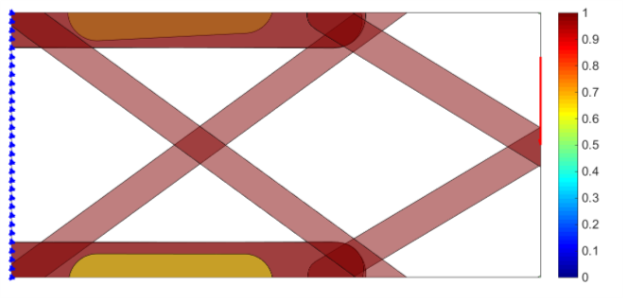
\includegraphics[width=0.45\linewidth]{figures/02_literature/coniglio1.png}}
    \hfill
    \subcaptionbox{}{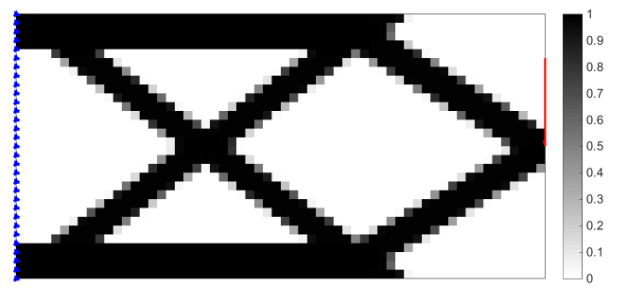
\includegraphics[width=0.45\linewidth]{figures/02_literature/coniglio2.png}}
    \hspace*{\fill}
    \caption{Component (a) and density (b) plot of a short cantilever beam optimized using the component-based topology optimization method \gls{ggp}~\cite{coniglio_generalized_2020}.}
    \label{fig:03_to_component}
\end{figure}

\subsection{Truss topology optimization (TTO)} \label{sec:02_tto}
\acrfull{tto} focuses on optimizing the topology of the truss structure itself, instead of operating on a continuous mesh. It involves selecting the cross-sectional areas and the connectivity of a discrete and dense mesh called ground structure, aiming to minimize weight while satisfying structural constraints. The process is graphically presented in \figref{fig:02_tto_ex}.

\begin{figure}
    \centering
    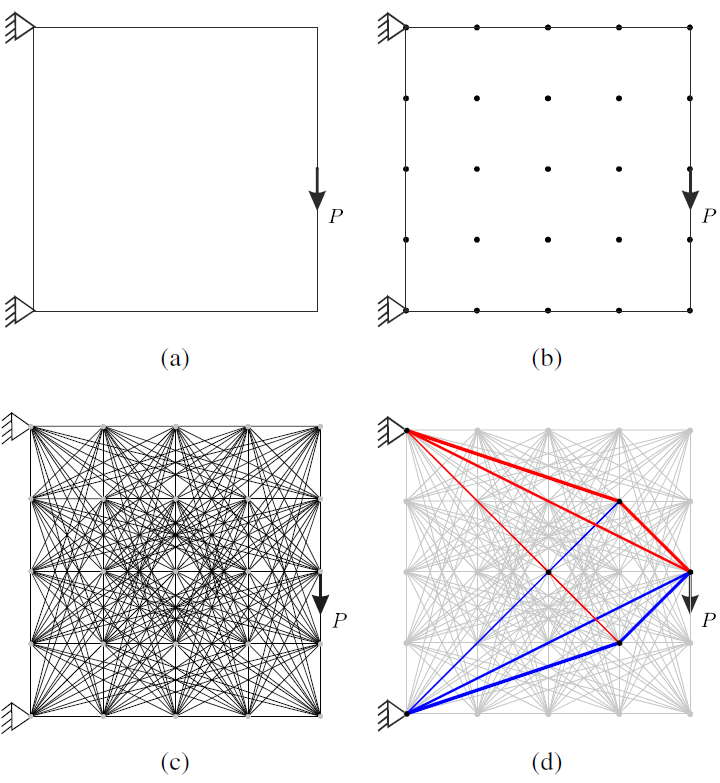
\includegraphics[width=0.7\linewidth]{figures/02_literature/layopt.png}
    \caption{The TTO algorithm can be divided into 4 steps: (a)
    specification of the design space, loads, and boundary conditions; (b) discretization
    of the design space; (c) the ground structure is generated depending on the
    desired connectivity level; (d) resolution of the optimization problem and plot of
    the solution \cite{he_python_2019}.}
    \label{fig:02_tto_ex}
\end{figure}

In the early works, the \gls{tto} problem was formulated in terms of member forces~\sidecite{dorn_automatic_1964, hemp_optimum_1973} with plastic material modelization, ignoring the kinematic compatibility to obtain a \gls{lp} problem. Formulated using the \gls{sand} approach, the equations of structural mechanics of the problem are imposed as constraints of the optimization and, contrary to \gls{nand} approaches, are not explicitly solved. Formulated that way, it is trivial to add maximum stress constraints compared to an equivalent \gls{nand} formulation. However, the \gls{sand} formulation with plastic material modelization only correctly predicts the mechanical behavior of statically determinate structures or mechanisms~\sidecite{kirsch_optimal_1989, rozvany_layout_1995}. Moreover, adding local buckling constraints to the optimization formulation is fundamental, as ultralight truss structures are often dominated by this mode of failure~\sidecite{sigmund_non-optimality_2016}. Multiple works in the field of truss structure optimization have focused on addressing these two crucial challenges~\sidecite{kirsch_optimal_1980,cheng_aspects_1995,achtziger_local_1999}.

\paragraph{Classical Michell structures} \label{sec:02_michell}
The characteristics of this class of truss structures are described by some simple criteria that date to the end of the 19th and the beginning of the 20th century. When a structure is statically determinate — \ie the structure is not a mechanism, and it is not over-constrained by the supports — the Maxwell theorem~\sidecite{maxwell_ireciprocal_1870} states that:
\begin{equation} \label{eq:02_maxwell-th}
    \sum_{\forall i | q_i>0}\ell_iq_i + \sum_{\forall i | q_i<0}\ell_iq_i = \textrm{const.}
\end{equation}
where $\ell_i$ and $q_i$ represent the length and the axial force of the $i$-th member, respectively. The constant value at the right of~\eqref{eq:02_maxwell-th} depends on the nature of the boundary conditions and the material used. The Maxwell theorem dictates that any increment in compression forces must be counterbalanced by an equivalent increase in tension forces when the structure remains topologically unchanged. So for statically determinate structures the structure layout is not influenced by the ratio between $\sigma_\text{c}$ and $\sigma_\text{t}$, Young's modulus $E$ of the material, nor the force magnitude.

Starting from Maxwell's findings, Michell theorized two further criteria for optimal truss structures~\sidecite{michell_limits_1904} valid when the maximum allowable stress is equal in tension and compression ($\sigma_\text{t} = \sigma_\text{c}$) and when the supports of the structure are statically determinate. The first one states that all the members of an optimal structure should present internal stress equal in magnitude to the maximum allowable value of the material -- \ie the structure is \textit{fully stressed}. The second criterion asserts that the strain of all the members of the structure should be equal and there should be no other point having a strain higher than this value. As formulated, these two criteria are known as the Michell criteria. The second criterion was later generalized by Hemp~\sidecite{hemp_optimum_1973} as:
\begin{equation} \label{eq:02_hemp}
    -\frac{1}{\sigma_\text{c}}\leq \varepsilon \leq \frac{1}{\sigma_\text{t}}.
\end{equation}
Compared to the second Michell criterion, \eqref{eq:02_hemp} permits the correct identification of the minimum volume structure even when different strength values for compression and tension and different support types are taken. These criteria are known as the Michell-Hemp criteria.

\paragraph{Plastic material formulation}
The rigid-plastic formulation characterizes the material as entirely rigid up to the point of reaching the yield stress, denoted as $\sigma_y$, and subsequently assumes a constant stress level of $\sigma_y$ once that threshold is exceeded. This formulation is a clear consequence of the application of the Michell-Hemp criteria and has thus been used in the very first work of \gls{tto}~\sidecite{dorn_automatic_1964,chan_optimum_1964,hemp_optimum_1973}. 

\paragraph{The ground structure approach}
The ground structure is a framework\marginnote{The first use of the ground structure in structural optimization is by Dorn \etal~\cite{dorn_automatic_1964}} composed of various structural members that connect specified points or nodes in two- or three-dimensional space (see \figref{fig:02_mesh_d}). These members can take the form of beams, columns, wires, or bar elements, depending on the specific structural requirements, but the most used is historically the bar element. Since the nodes within the ground structure are considered as pin-joints, all straight members exclusively face either tension or compression loads. 
\begin{marginfigure}
    \centering
    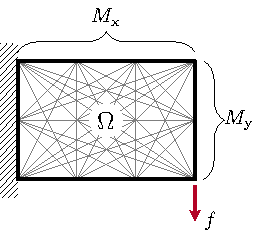
\includegraphics{figures/02_literature/04_disc_mesh/d_mesh.pdf}
    \caption{The domain $\Omega$ is discretized using a set of straight members connecting a set of nodes. This framework is known as the ground structure.}
    \label{fig:02_mesh_d}
\end{marginfigure}

Depending on how the connectivity of the grid of nodes is, we can experience very different ground structures. In a fully connected ground structure, every node within the system is linked to every other node, resulting in a dense and redundant structural configuration. The number of bars $N_{\text{el}}$ of a fully connected ground structure can be determined using the following formula:
\begin{equation}
    N_{\text{el}} = \frac{M \cdot (M-1)}{2},
\end{equation}
where $M$ represents the number of nodes of the structure.

In classic works, the ground structure is used as the start of the optimization, where the optimized structure is obtained as a subset of the initial ground structure, but multiple alternative approaches have been proposed since then, \eg starting from a very coarse ground structure that is enriched during the analysis~\sidecite{gilbert_layout_2003}, or giving the nodes of a coarse ground structure the possibility to move, during~\sidecite{pedersen_optimal_1973, achtziger_simultaneous_2007, descamps_lower-bound_2013}, or after the optimization, simultaneously reducing the number of active members of the solution~\sidecite{he_rationalization_2015, lu_reducing_2023}. Recently, a hybrid method based on the projection of explicitly defined components on a discrete ground structure has been proposed, easing the interpretation of the stiffening pattern of the optimized truss \sidecite{savine_component-based_2021}.

\paragraph{Optimization formulation}
The volume minimization formulation with maximum stress constraints is stated in terms of members' cross-sectional areas $\vect{a}$ and member forces $\vect{q}$ as follows:
\begin{equation}
    \begin{aligned}
    \min_{\vect{a}, \vect{q}}   && V &= \vect{\ell}^{T}\vect{a} && \textrm{(Volume minimization)}\\
    \textrm{s.t.}   && \matr{B}\vect{q} &= \vect{f} && (g_\text{eq})\\
    && -\sigma_\text{c}\vect{a} &\leq \vect{q} \leq \sigma_\text{t}\vect{a} && (g_\text{st,c}, \; g_\text{st,t}) \\
    && \vect{a} &\geq 0, \\
    \end{aligned}
    \tag{$\mathbb{P}_0$}
    \label{eq:02_optim_original}
\end{equation}
where $\matr{B}$ is a $N_{\text{dof}} \times N_{\text{el}}$ matrix containing the direction cosines of the $i$-th member with respect to the $i$-th degree of freedom to calculate the nodal force equilibrium constraints $\vect{g}_\text{eq}$, and where $N_{\text{dof}}$ is the number of \gls{dofs}, equal to $2M$ or $3M$ for a two- or a three-dimensional load case, respectively. $\vect{q} = [q_1, q_2, \ldots,q_{N_{\text{el}}}]^T$ is the vector containing the internal member forces, with a positive sign when in tension, caused by the external load $\vect{f} = [f_1, f_2, \ldots,f_{N_{\text{dof}}}]^T$. The state variable $\vect{a} = [a_1, a_2, \ldots,a_{N_{\text{el}}}]^T$ represents the cross-sectional area of the $N_{\text{el}}$ members of the structure. $\sigma_\text{c}$ and $\sigma_\text{t}$ are the compressive and tensile maximum allowable stresses of the material, respectively, used in the stress constraints $\vect{g}_\text{st,c}$ and $\vect{g}_\text{st,t}$. This formulation takes into account only the linear behavior of the structure and is equivalent to the original and well-studied member force formulation~\sidecite{dorn_automatic_1964, bendsoe_topology_2004}.

The resolution of Problem \ref{eq:02_optim_original} frequently produces complex structures made up of a multitude of small members that tend to the shapes of Michell structures (see Fig~\ref{fig:02_truss-ex})~\sidecite{michell_limits_1904}. While it is known that these structures are nearly optimal, one would want to limit the complexity of the resulting structure. Substituting $\vect{\ell}$ with $\vect{\tilde{\ell}} = [\ell_1 + s, \ell_2 + s, \ldots,\ell_{N\text{el}} + s]^T$ in the objective function of \ref{eq:02_optim_original}, one would penalize the appearance of small members~\sidecite{parkes_joints_1975}. $\vect{\tilde{\ell}}$ is called augmented member length and $s$ the joint cost. This approach mimics the mesh-independency regularization filter of topology optimization, avoiding the inevitable apparition of structures with tiny features when a fine mesh is adopted.

\begin{marginfigure}
    \centering
    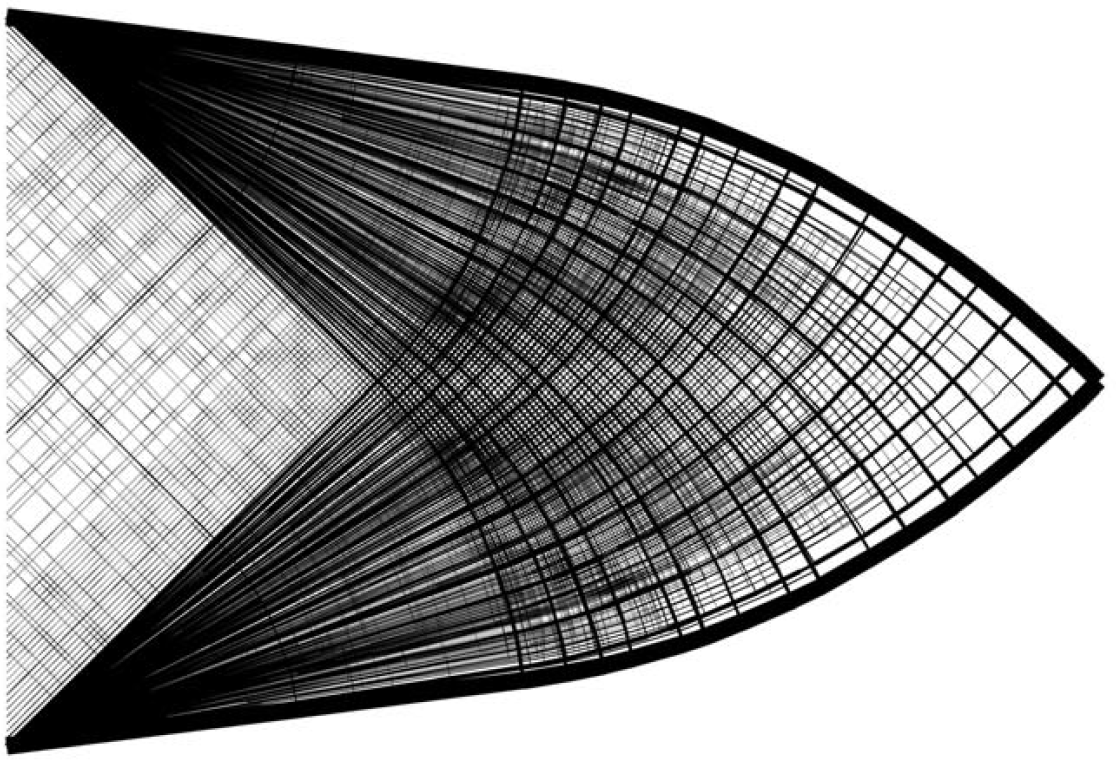
\includegraphics[width=\linewidth]{figures/02_literature/truss-ex.png}
    \caption{The optimal structures found by layout optimization tend at Michell-like structures, made up of a very large number of infinitesimal struts \cite{gilbert_layout_2003}.}
    \label{fig:02_truss-ex}
\end{marginfigure}

\section{Modular structures and lattice materials}
Historically, material properties were modified by manipulating chemical composition, microstructure, and production processes \sidecite{schaedler_architected_2016}. Another possible way to enhance material properties involves tailoring the spatial arrangement of solids and voids within the material. Referred to as architected materials, this concept has gained significant traction in research, particularly with recent advancements in additive manufacturing. These materials, often observed in natural structures like bone microstructures or birds' beaks (refer to \figref{fig:02_nature} for additional examples), have garnered interest due to the recognition that optimal structures exhibit stiffness across multiple scales~\sidecite{kohn_optimal_1986,allaire_optimal_1999}. Additionally, Fleck noted~\sidecite{fleck_micro-architectured_2010} that one reason for structural hierarchy in engineering is to augment buckling strength. Local buckling strength scales with the strut length $l$ following $l^{-2}$, indicating that finer length scales contribute to higher buckling strength.

\begin{figure}
    \subcaptionbox{}{
\includegraphics[width=0.45\linewidth ]{figures/02_literature/1.jpg}}
    \hfill
    \subcaptionbox{}{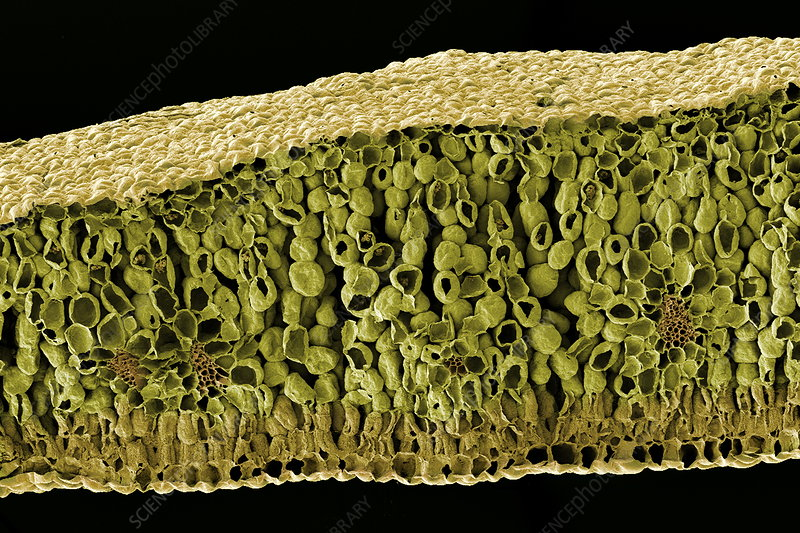
\includegraphics[width=0.45\linewidth ]{figures/02_literature/3.jpg}}
    \bigskip
    \subcaptionbox{}{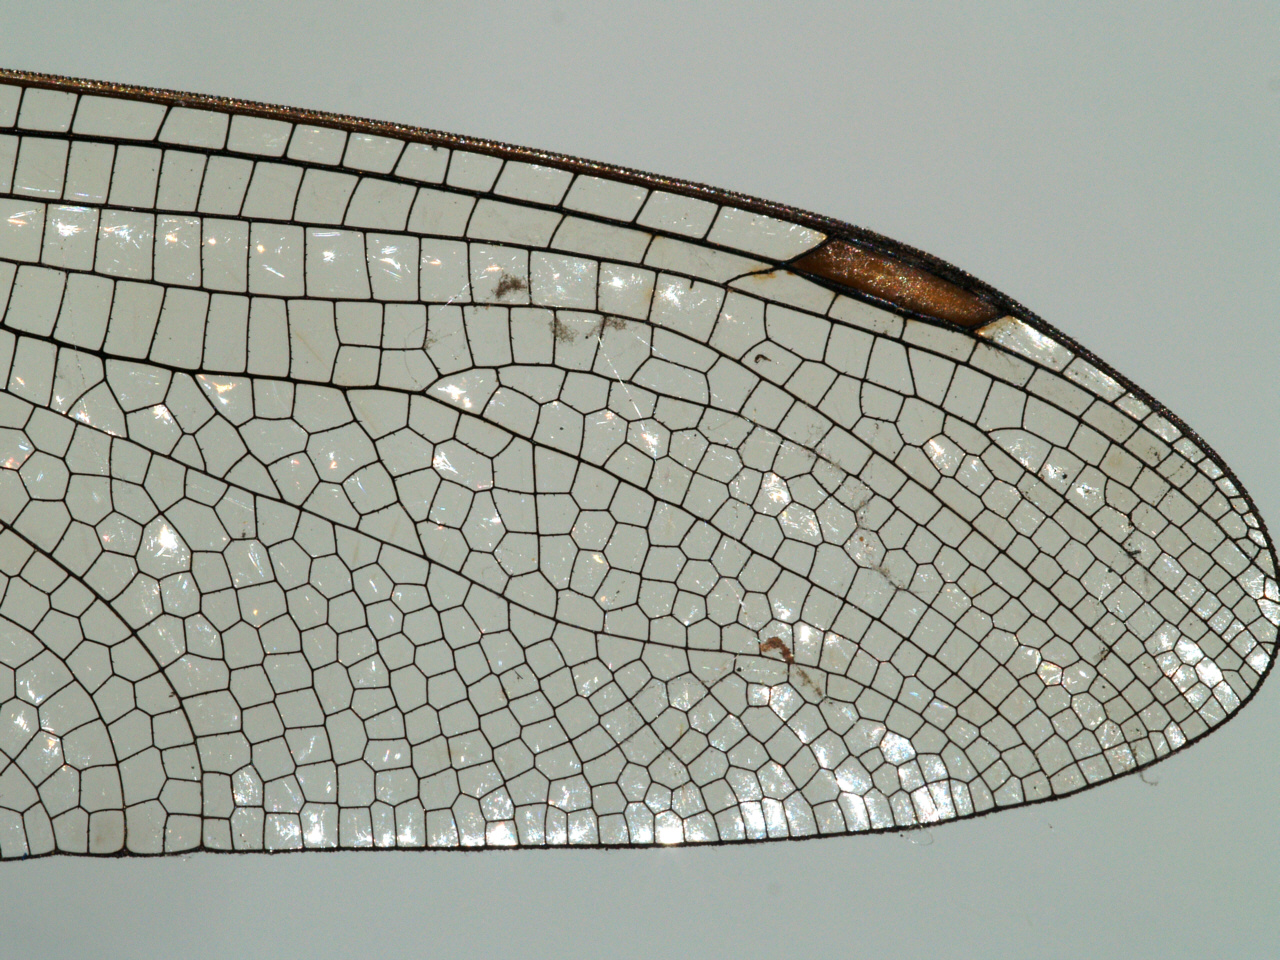
\includegraphics[width=0.45\linewidth ]{figures/02_literature/2.jpg}}
    \hfill
    \subcaptionbox{}{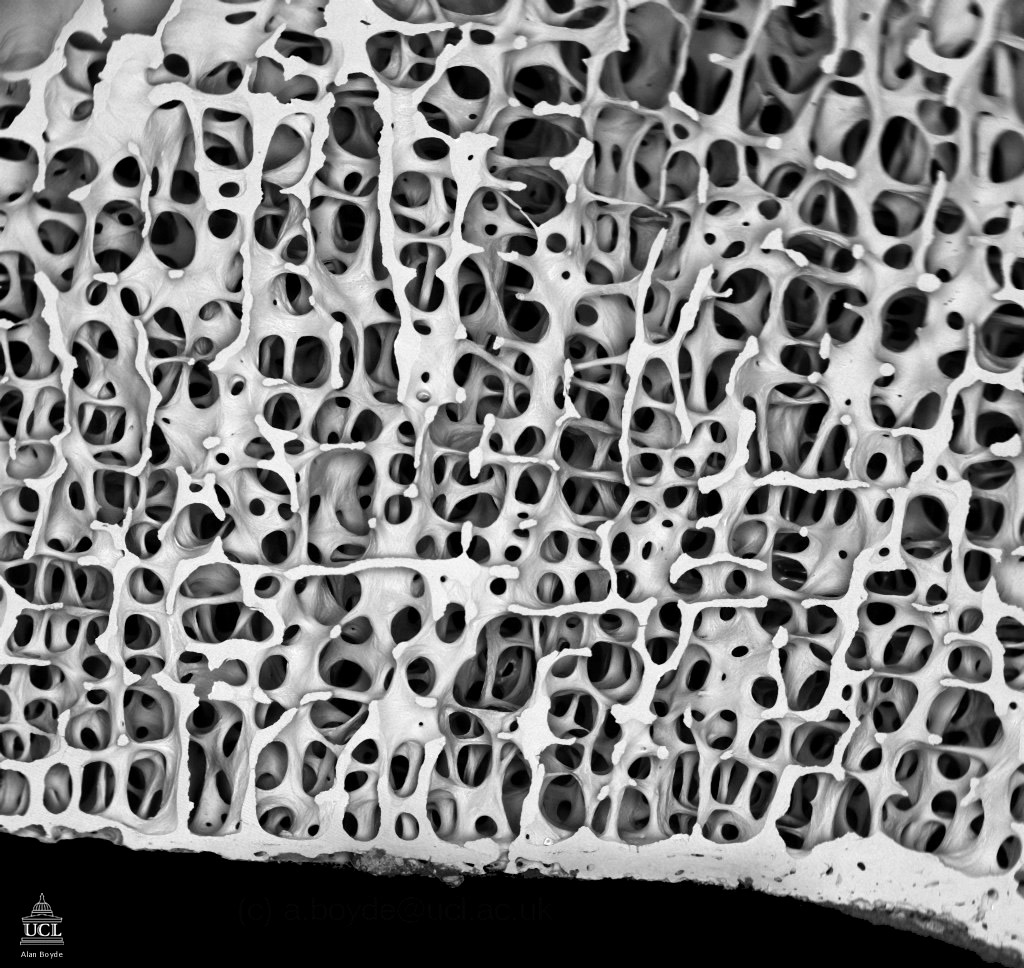
\includegraphics[width=0.45\linewidth ]{figures/02_literature/4.jpg}}
    \caption{The natural evolution process frequently generates lattice materials and modular structures; (a) The spore-bearing gills of a Hypholoma fasciculare \cite{nz_hypholoma_2023} (b) SEM image of a leaf microstructure \cite{library_leaf_nodate} (c) cellular stucture of the wing of a dragonfly \cite{gripspix_mostly_off_health_issues_wing_2007} (d) internal structure of a human bone \cite{noauthor_bone_03_nodate}.}
    \label{fig:02_nature}
\end{figure}

If we observe the Ashby material chart~\sidecite{ashby_materials_1999} shown in \figref{fig:02_ashby_ch}, where the material yield strength is plotted against density, it becomes evident that numerous empty spaces exist. Besides some unattainable areas delineated by the \gls{hs} bounds\sidenote{The \gls{hs} bounds are the tightest bounds possible from the range of composite moduli for a two-phase isotropic mixture. In lattices, usually, the second material is void.}, these empty spaces can be filled by architected structures, extending the property space of actual materials.
\begin{figure}
    \centering
    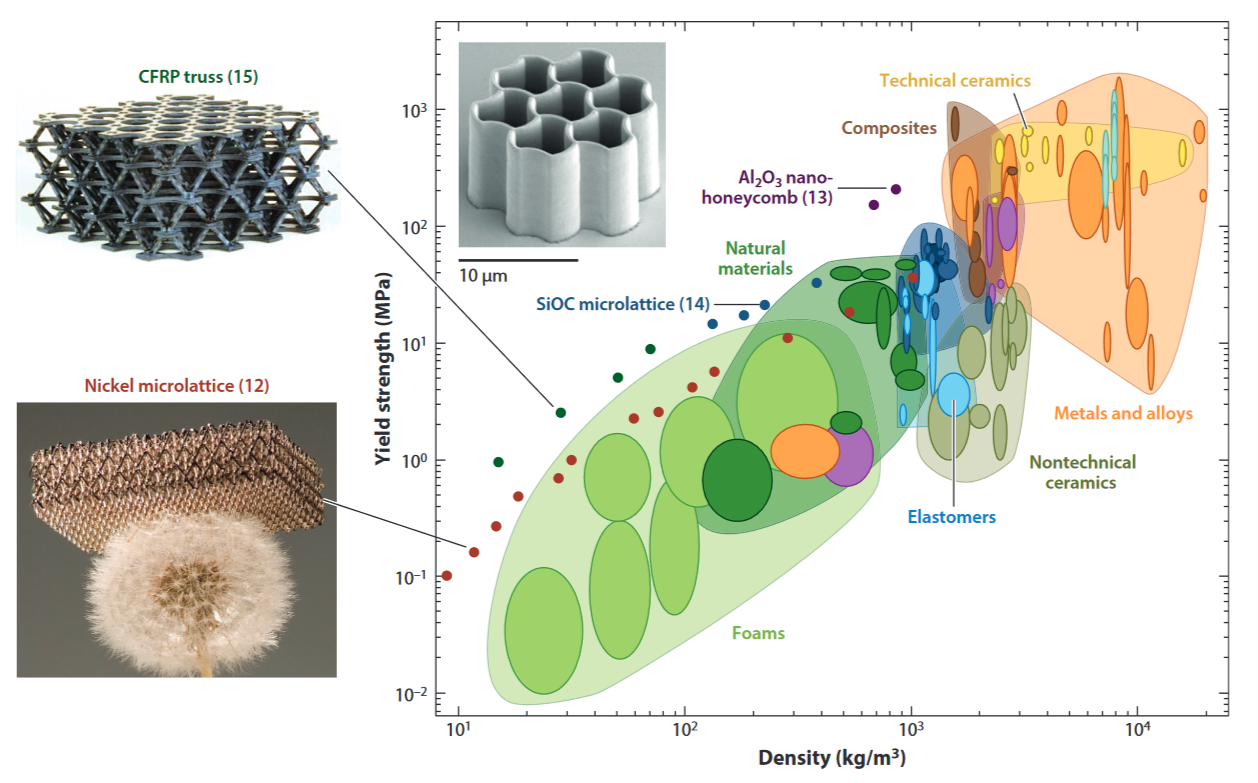
\includegraphics[width=\linewidth]{figures/02_literature/ashby_chart.png}
    \caption{Density versus yield strength Ashby chart. Exploiting the architecture of the material as a variable to design new metamaterials, empty spaces of the graph can be filled (see dots) \cite{schaedler_architected_2016}.}
    \label{fig:02_ashby_ch}
\end{figure}

A highly interesting class of architected materials and structures is represented by lattices, alternatively referred to in the literature as cellular architected or modular materials and structures. The defining feature of lattices is to exhibit a repetitive \gls{rve} (also commonly called module or cell) that is replicated throughout space. This characteristic allows for the establishment of a systematic and reproducible unit that captures the essential structural and material properties of the lattice. The study of the repetitive nature of the \gls{rve} permits a comprehensive understanding of the lattice's behavior, enabling researchers to analyze and predict its mechanical, thermal, and other pertinent properties with a high degree of accuracy~\sidecite{bensoussan_asymptotic_1978}. It is possible to differentiate between a lattice material and a lattice structure based on the size of the \gls{rve} with respect to the considered structure. In a lattice structure, there is no clear physical scale separation between the \gls{rve} and the macrostructure, indicating that the lattice's characteristics are manifested at both the micro and macro scales (see \figref{fig:02_madcat}). However, defining a specific threshold to distinctly categorize the two is challenging, as the transition from lattice material to lattice structure can be gradual and context-dependent~\sidecite{dai_size_2008,kalamkarov_asymptotic_2009,coelho_scale-size_2016,zhang_multiscale_2018}.

\begin{figure}
    \centering
    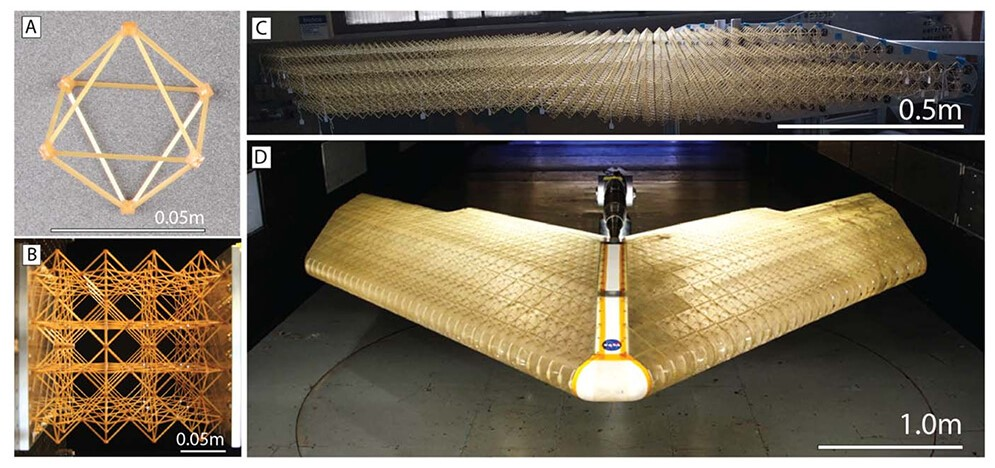
\includegraphics[width=\linewidth]{figures/02_literature/nasa-madcat-morphing-wing-breakdown-1000-x-600(1).jpg}
    \caption{The different length scales present in a modular structure~\cite{cramer_elastic_2019}. The size of the \gls{rve} is comparable with the dimensions of the wing, especially in the thickness. We therefore talk about modular structure and not lattice material.}
    \label{fig:02_madcat}
\end{figure}

Lattice structures and materials exhibit a wide range of promising applications. They showcase notable energy-absorbing properties, particularly when designed as bending-dominated structures~\sidecite{evans_concepts_2010,schaedler_designing_2014,ozdemir_energy_2016}. This quality positions lattice structures as potential candidates for a novel design scheme in aerodynamics, thanks to their remarkable aeroelastic properties~\sidecite{opgenoord_aeroelastic_2018,cramer_elastic_2019}. Additionally, lattices have proven to be compelling choices for constructing biomedical scaffolds~\sidecite{hutmacher_scaffolds_2000,mota_additive_2015,nikolova_recent_2019}. Furthermore, lattice materials demonstrate excellent heat exchanger properties, attributed to their high surface-to-volume ratio and the turbulent mixing flow they induce when a fluid passes through~\sidecite{lu_heat_1998,wadley_thermal_2007}.
\begin{marginfigure}
        
\includegraphics[width=\linewidth]{figures/02_literature/wellington.jpg}
        \caption{Vickers Wellingtons, bombers utilized during World War II, remained operational despite sustaining extensive damage, thanks to their lattice fuselage. When one of the ribs was damaged, the load was redistributed to the others, allowing the structure to remain functional \cite{airshowconsultants_real_2013}.}
        \label{fig:vick}
\end{marginfigure}
\begin{marginfigure}
    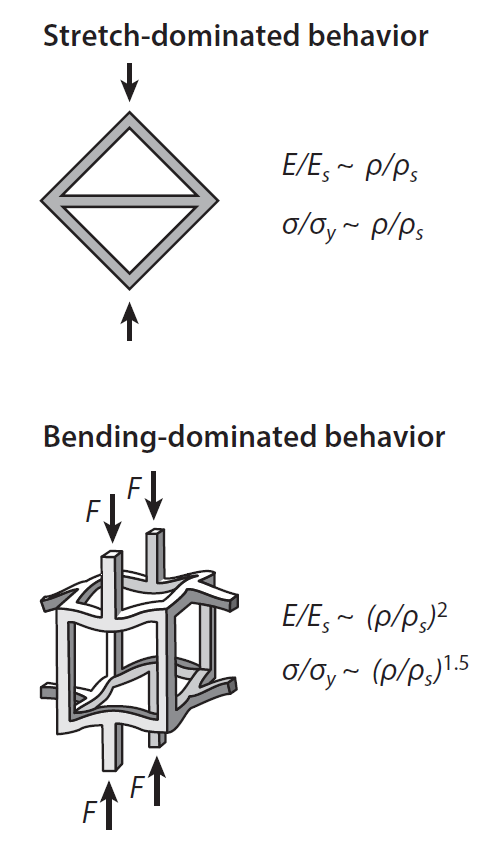
\includegraphics[width=\textwidth]{figures/02_literature/stretc-bend.png}
    \caption{A stretch-dominated and a bending-dominated \gls{rve}. Bending-dominated structures act as a mechanism if the joints cannot withstand moments. The scaling laws are different for the two structure families \cite{schaedler_architected_2016}.}
    \label{fig:02_str_bend}
\end{marginfigure}
Lattices show additional captivating properties that demonstrate their versatility. Firstly, modular structures can be purposefully designed for reversible assembly, introducing the concept of rapid assembly and easily repairable structures. Various approaches, such as utilizing fasteners~\sidecite{cheung_reversibly_2013,jenett_digital_2017,cramer_elastic_2019}, or incorporating snap-fit joints~\sidecite{dong_mechanical_2015}, have been proposed to realize this idea. Furthermore, lattice structures inherently exhibit damage tolerance~\sidecite{stolpe_fail-safe_2019,wu_topology_2021}. In a skin-lattice design, the skin is non-load-bearing, ensuring that skin damage does not lead to progressive structural failure. Additionally, in cases of rib damage, the affected rib can be isolated from the load without compromising the integrity of the entire structure (refer to Fig.~\ref{fig:vick}). Lastly, lattice structures pave the way for extensive utilization of robotics in both the manufacturing~\sidecite{hunt_wraptor_2019} and assembly phases~\sidecite{gershenfeld_macrofabrication_2015,jenett_bill-e_2017,costa_algorithmic_2020,niehs_recognition_2020}.

Lattices can be categorized as open- or closed-wall structures based on the topology of the repeating \gls{rve}. Despite closed-wall lattices potentially resulting in stiffer structures, the preference for open-cell configurations is well-articulated by Sigmund \etal~\sidecite{sigmund_non-optimality_2016}. They emphasize that the outcome of minimum compliance-type continuum topology optimization studies should inherently be of sheet type unless explicit constraints favoring Michell-like structures are specified. These constraints include considerations of structural and microstructural stability, where the load required to initiate buckling in a slender strut of an open-cell lattice is significantly higher than that of a comparable closed-cell lattice~\sidecite{deshpande_foam_2001}. Consequently, open-cell structures are less prone to buckling. Additionally, the porosity of open-wall cells allows for the passage of flow, making them suitable for applications such as heat exchangers or promoting bone regrowth in biomedical scaffolds. From a manufacturing perspective, open-cell designs are preferable, as very thin walls are challenging to manufacture. The transparency inherent in open-cell structures is advantageous for tasks such as repair and health monitoring. Finally, an open-cell design is considered elegant and aesthetic, as it embodies Michell-like structures, which are described as "inarguably beautiful" and "look elegant and efficient" by Sigmund \etal~\cite{sigmund_non-optimality_2016}.

Lattice structures are further categorized into stretching- and bending-dominated based on the \gls{rve} topology. A stretching-dominated structure is characterized as a lattice in which its constitutive struts exclusively experience tension and compression loads. In such a structure, the nodal stiffness does not contribute to the overall structural stiffness, and the truss undergoes collapse primarily through the stretching of its struts. Desphande \etal~\cite{deshpande_foam_2001} noted that freezing the joints of a stretching-dominated truss has minimal impact on its macroscopic stiffness or strength. Despite the bending of the struts, the frame remains stretching-dominated, and the collapse load is predominantly determined by the axial strength of the struts. Consequently, if an open-cell structure is stretching-dominated, it can effectively be treated as a connected set of pin-jointed struts.

The relative density of the lattice is defined as:
\begin{equation}
    \bar{\rho} = \frac{\rho_l}{\rho}
\end{equation}
where $\rho_l$ and $\rho$ represent the density of the lattice and the dense material, respectively~\sidecite{ashby_properties_2006}. A stretching-dominated structure exhibits approximately 10 times greater stiffness and 3 times greater strength than a bending-dominated structure at $\bar{\rho} = 0.1$, as illustrated in Figure~\ref{fig:02_str_bend}~\cite{deshpande_foam_2001}. Nevertheless, when subjected to compression, stretching-dominated structures display a softening post-yield response attributed to the buckling of struts, rendering them less suitable for energy absorption tasks. In contrast, bending-dominated lattices showcase a more favorable energy-absorbing behavior, characterized by a plateau-like response.

\subsection{Modular structures and lattice materials optimization}
The initial density-based topology optimization method, as seen in Bendsøe and Kikuchi's foundational work~\sidecite{bendsoe_generating_1988}, employed numerical homogenization to model a meta-material consisting of infinitesimally small square cells with square holes. Notably, this marked the advent of multi-scale optimization, driven by the observation that optimal stiffness for a structure encompasses various scales \sidecite{kohn_optimal_1986,allaire_optimal_1999}.

In the 1990s, the focus shifted from homogenization algorithms to mono-scale algorithms, where the optimization involved a homogeneous distribution of an isotropic material \sidecite{bendsoe_optimal_1989,zhou_coc_1991}. This shift was primarily caused by the manufacturing challenges associated with producing multi-scale meta-materials. Subsequently, these approaches evolved into what is now known as density-based topology optimization. Mono-scale methods, where the design domain discretization results in structures at a single scale, can achieve theoretical stiffness-optimal structures spanning multiple scales with fine mesh discretization and careful continuation techniques, provided there is no regularization for mesh independence. Bendsøe and Kikuchi's original work and homogenization-based algorithms have gained recently more interest due to the advances in additive manufacturing technologies. Contemporary studies are combining asymptotic homogenization and topology optimization to optimize multi-scale structures. 

Lattice structures are optimized through either a multi-scale or a full-scale approach. Multi-scale algorithms operate on structures with different physical scales between the micro- and macro-levels, assuming periodic boundary conditions for the \gls{rve}. Doing that allows for the use of a material model with micro-structure properties evaluated using asymptotic homogenization. In contrast, full-scale methods represent mono-scale approaches where optimization is achieved by directly controlling the layout locally. In these full-scale approaches, both analysis and optimization are conducted at the full resolution of the domain. For a more in-depth exploration and comparison of full-scale and multi-scale approaches, interested readers can refer to the comprehensive review by Wu \etal \sidecite{wu_topology_2021}.

\subsection{Multi-scale structures optimization}
Multi-scale topology optimization approaches aim to speed up computations for optimizing structures at full resolution. Optimal structures span multiple scales, and using a finer mesh allows for detailed geometric improvements, potentially enhancing optimized structures. However, higher-resolution mono-scale approaches come with increased computational costs. To tackle this, multi-scale approaches like the hierarchical method by Rodrigues \etal~\sidecite{rodrigues_hierarchical_2002} and de-homogenization techniques~\sidecite{pantz_post-treatment_2008, groen_homogenization-based_2018} have been introduced.

The hierarchical optimization framework consists of a master problem addressing the global spatial distribution of material and an inner problem tackling the optimal choice of material at the local level. This approach shifts the focus from a specific composite's material distribution problem to a more comprehensive challenge involving both topology and material optimal design. The idea is to use the homogenized micro-scale cell as the base material of the macro-scale topology optimization. \figref{fig:02_homogen} gives a graphical representation of how asymptotic homogenization works.
\begin{figure}
    \centering
    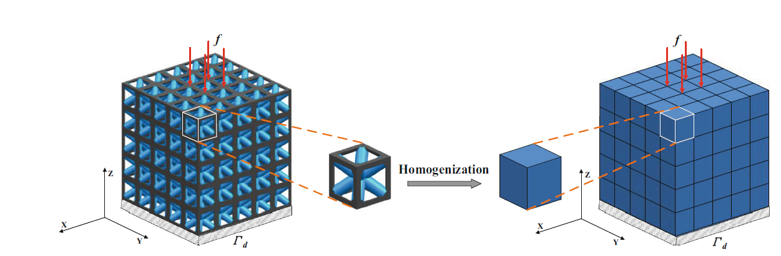
\includegraphics[width=\linewidth]{figures/02_literature/homo.png}
    \caption{Graphical representation of the asymptotic homogenization method used to retrieve the equivalent mechanical properties of a periodic cell \cite{wang_concurrent_2020}.}
    \label{fig:02_homogen}
\end{figure}
The equivalent elastic tensor $\mathbf{C}^{H}$ is calculated using the following formula~\sidecite{guedes_preprocessing_1990}:
\begin{equation}
    \mathbf{C}^{H}=\frac{1}{\left|\Omega_{m}\right|} \int_{\Omega_{m}} \left(\varepsilon_{m}^{0}-\varepsilon_{m}\right)\mathbf{C}\left(\varepsilon_{m}^{0}-\varepsilon_{m}\right) d \Omega_{m}
\end{equation}
where $\mathbf{C}^{H}$ is the homogenized elastic tensor, $\Omega_{m}$ represents the \gls{rve} volume, $\mathbf{C}$ is the base material elastic tensor and $\varepsilon_{m}^{0}$ are called unit test strain and are defined as $\boldsymbol{\varepsilon}^{11}=(1,0,0)^{T}, \boldsymbol{\varepsilon}^{22}=(0,1,0)^{T}, \boldsymbol{\varepsilon}^{12}=(0,0,1)^{T}$. An example of the results obtained using a hierarchical method is presented in \figref{fig:02_hierarchical}.
\begin{figure}
    \centering
    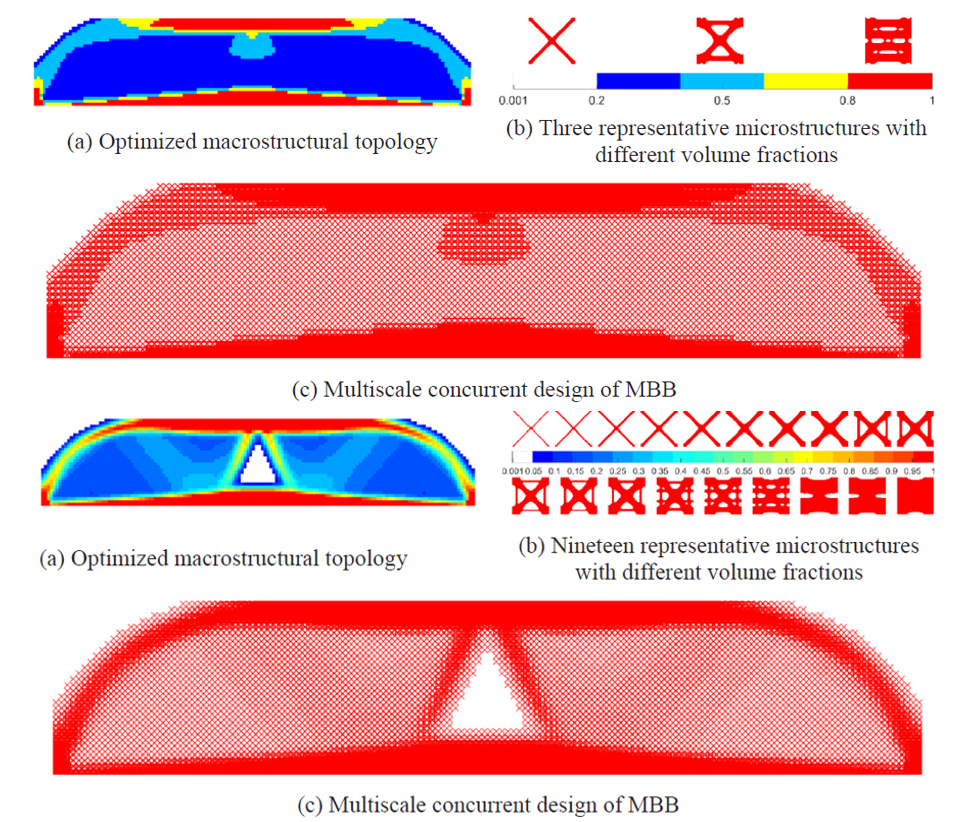
\includegraphics[width=0.9\linewidth]{figures/02_literature/top_multiscale.png}
    \caption{In the study of Zhang \etal \cite{zhang_multiscale_2018} the same test case is optimized using a different number of microstructures. Here we show the multi-scale optimized structures using 3 and 19 different microstructures.}
    \label{fig:02_hierarchical}
\end{figure}

De-homogenization is an approach where the optimization problem is initially solved solely on the macroscopic level using a homogenization method. Subsequently, an additional phase is introduced to obtain connected and physically realizable microstructures based on the obtained macroscopic result. In the macroscale optimization, multiple additional parameters are typically optimized concurrently with the density of the Representative Volume Element (\gls{rve}). These parameters may include microstructure orientation, contributing to the creation of a smooth mapping function \sidecite{groen_homogenization-based_2018,allaire_topology_2019,geoffroy-donders_3-d_2020,kumar_density-and-strain-based_2020}. An alternative approach involves approximating the material behavior through a reduced database model, as demonstrated by Xia and Breitkopf \sidecite{xia_multiscale_2015}. In this method, microstructural computations are performed offline, only once. Precomputed databases are often employed to obtain the full design for the parametrized lattice \gls{rve}, often using a polynomial model to interpolate between the database microstructures \sidecite{wang_concurrent_2018,imediegwu_multiscale_2019}. Recent approaches are now using \gls{ai} and deep learning to speed up the de-homogenization phase~\sidecite{kim_machine_2021,white_multiscale_2019,chandrasekhar_multi-material_2021,wang_enhancing_2021} 

In conclusion, despite maintaining the separation of the two physical scales during the optimization process, it is imperative to conduct a full-scale validation for all multi-scale methods, as highlighted in various studies \sidecite{groen_homogenization-based_2018,wu_topology_2021, duriez_well_2021, sigmund_benchmarking_2022}. Additionally, the multi-scale optimization approaches in which the microstructure is aligned to local stress fields without constraints imposed by cell geometry or orientation \sidecite{groen_homogenization-based_2018}, deliver good performance even for structures with less periodicity compared to a bulk distribution.

\subsection{Full-scale structures optimization}
\begin{figure*}
    \centering
    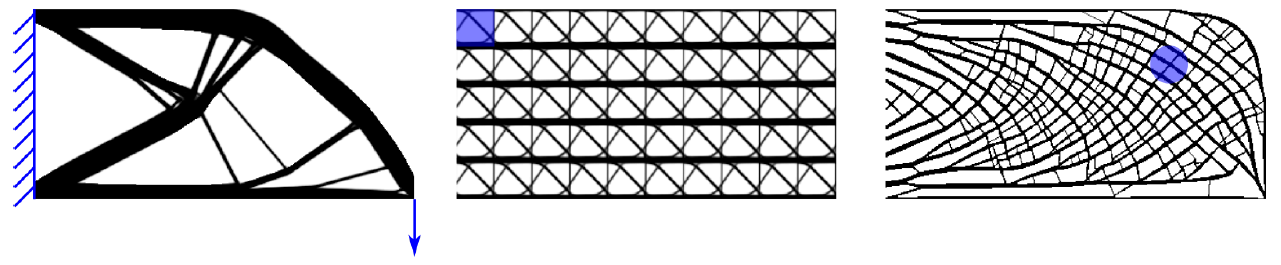
\includegraphics[width=0.8\linewidth]{figures/02_literature/full-to.png}
    \caption{Three structures with the same volume are optimized for compliance minimization using three different methods: on the left, a classic mono-scale topology optimization algorithm. Middle: the variable linking method is used to enforce the pattern repetition on the structure. On the right an optimized structure with local volume constraints. The algorithms used to optimize the last two structures belong to the family of \textit{full-scale} methods. \cite{wu_topology_2021}.}
    \label{fig:02_full-to}
\end{figure*}

Recent studies have focused on assessing homogenization predictions compared to mechanical responses, revealing up to a \qty{20}{\percent} variation in the effective components of the stiffness tensor for a $6\times6\times6$ cube when compared to homogenized models \sidecite{coelho_scale-size_2016,cheng_functionally_2019}. This variability is attributed to the "boundary layer phenomenon" observed in the late 70s, challenging the assumptions of periodic boundary conditions and scale separability inherent in homogenization \sidecite{bensoussan_asymptotic_1978,kalamkarov_asymptotic_2009}. To address these limitations, a new family of methodologies, known as full-scale approaches, has emerged. Unlike homogenization-based methods, full-scale approaches, such as pattern repetition (also known as variable linking) and local volume constraints, avoid reliance on homogenization. In pattern repetition, the initial design space is partitioned into repetitive domains that are optimized and constrained to ensure their uniformity \sidecite{zhang_scale-related_2006}. In contrast, the local volume constraints method imposes an upper limit on the solid elements' fraction in a neighborhood radius centered at each point within the design domain. The objective is to generate porous structures aligned with principal stress directions. While experiencing a modest stiffness reduction compared to mono-scale designs, these structures demonstrate heightened resilience against variations in load angle, local material failure, and buckling \sidecite{wu_infill_2018}.

Variable linking approach faces a common limitation, leading to compromised structural performance due to topological periodicity~\sidecite{zhang_scale-related_2006,huang_optimal_2008}. This limitation arises as the design converges toward solutions influenced by the region with the highest compliance, resulting in suboptimal solutions for other regions where the same module design is applied~\sidecite{tugilimana_integrated_2019}. To address this, Bakker~\sidecite{bakker_simultaneous_2021} identified two key approaches. The first involves extending the solution space by introducing additional module properties as design variables. For instance, allowing module rotations has proven effective, as it modifies the local material distribution and enhances structural performance~\sidecite{tugilimana_spatial_2017}. Another extension involves allowing the module unit to resize, providing flexibility in adapting to different regions within the global domain~\sidecite{stromberg_application_2011,wu_system_2016}. These strategies offer ways to overcome the challenges associated with topological periodicity and achieve more optimal solutions for diverse regions within the structure.